\documentclass{article}
\usepackage[utf8]{inputenc}
\usepackage[T1]{fontenc}
\usepackage{hyperref}
\usepackage{todonotes}
\usepackage{gensymb} % superscript
\usepackage{textcomp} % superscript
\usepackage{amsmath} % symboles des degrés

% --------------------  NOMBRES ET UNITÉS ---------------------------
\usepackage{siunitx}
\iffalse % explication des fonctions courantes
The package provides the user macros:
• \ang[hoptionsi]{hanglei}
• \num[hoptionsi]{hnumberi}
• \si[hoptionsi]{huniti}
• \SI[hoptionsi]{hnumberi}[hpre-uniti]{huniti}
• \numlist[hoptionsi]{hnumbersi}
• \numrange[hoptionsi]{hnumbersi}{hnumber2i}
• \SIlist[hoptionsi]{hnumbersi}{huniti}
• \SIrange[hoptionsi]{hnumber1i}{hnumber2i}{huniti}
• \sisetup{hoptionsi}
• \tablenum[hoptionsi]{hnumberi}
plus the S and s column types for decimal alignments and units in tabular environments.
12 345.678 90        \num{12345,67890}
1 ± 2i               \num{1+-2i}
0.3 × 1045           \num{.3e45}
1.654 × 2.34 × 3.430 \num{1.654 x 2.34 x 3.430}

\si{kg.m.s^{-1}}
kg m s−1
Simple lists and ranges of numbers can be handled.
\numlist{10;20;30} \\
\SIlist{0.13;0.67;0.80}{\milli\metre} \\
\numrange{10}{20} \\
\SIrange{0.13}{0.67}{\milli\metre}
10, 20 and 30
0.13 mm, 0.67 mm and 0.80 mm
10 to 20
0.13 mm to 0.67 mm

\ohm\metre
\celsius

\fi
% --------------------------------------------------------------

\usepackage{hyperref}

\usepackage{natbib}       % Pour la bibliographie
\usepackage[french]{babel}
\usepackage{graphicx}     % Pour les figures
\usepackage[toc]{appendix}% Pour les annexes
\usepackage{titlesec}     % Pour modifier les titres
\usepackage{fancyhdr}     % Pour les haut et bas de pages (numéros)
\usepackage{lipsum}       % Rajoute du texte temporaire
\usepackage{parskip}      % Modifie l'apparence des paragraphes
\usepackage{setspace}     % Pour interligne et demi
\usepackage{listings}     % Pour afficher du code sans formattage

\selectlanguage{french}

% ------------------------- COMMANDES -------------------------------

\newcommand\var[2]{\newcommand{#1}{\ensuremath{#2}}}
% C'est pratique de définir des variables au début pour éviter de
% réécrire des formules et cela facilite modifier l'affichage.

\makeatletter
\newcommand{\makecustomtitle}{
  \newpage
  \null
  \begin{center}
  \let \footnote \thanks
    {\LARGE \textbf{\@title} \par}
    \vskip 1em
    {\large \@date \par}
    \rule{1.5in}{0.4pt}
  \end{center}
  \par
}
\makeatother


\title{Four à aluminium}
\author{Pascal Rainville }
\date{Décembre 2018}

\usepackage[top=0.5in]{geometry}

\begin{document}

\makecustomtitle

\section{Introduction}

Un four de fondrie sert à faire fondre des métaux afin de pouvoir les mouler. Ce document présente un modèle à résistance électrique. C'est un élément chauffant qui produit la chaleur.

\section{Fabrication}

Des briques sont collées ensemble avec un ciment haute température.

Un petit frame de métal avec deux poignées est fabriqué afin de transporter le four. Le but étant de pouvoir soulever plus facilement le four. La brique est peu résistante en tension. Le four ne peut pas être pris par les murs. Il doit être soulever par la base.

\subsection{Élément chauffant V2}

La résistance électrique de l'élément doit être suffisament petite afin de laisser passer du courant d'une puissance de 1200 Watts. (Pour référence, un grille-pain utilise 900 Watts)

L'élément a été coupé pour bien rentré dans l'espace disponible. Il possède une résistance de 8 ohms. Le voltage requis est

\begin{equation} \label{eq:1}
    E = \sqrt{PR}
\end{equation}
\[E = \sqrt{(\SI{1200}{W})(\SI{8}{\ohm}})\]
\[\boxed{E = \SI{98}{V}}\]

Le voltage requis est inférieur au voltage disponible (ici 120 V). Un diviseur de tension est ainsi utilisé pour limité la tension.

\todo{Rajouter un diagramme qui montre un diviseur de tension}

\[I = \frac{E}{R_1+R_2}\]
\[E_{R_1} = IR_1\]
\[E_{R_1} = E\frac{R_1}{R_1+R_2}\]
\begin{equation} \label{eq:2}
    R_2 = R_1(\frac{E}{E_{R_1}}-1)
\end{equation}

L'équation \ref{eq:1} avec l'équation \ref{eq:2} donne
\begin{equation}
        R_2 = R_1(\frac{E}{\sqrt{P(\SI{8}{\ohm})}}-1)
\end{equation}

Pour P = 1200 Watts,
\[R_2 = 0.2245R_1\]

Pour P = 100 Watts,
\[R_2 = 3.2426R_1\]

Je vais essayer autour de 100 Watts et on va voir.

\begin{figure}[ht]
    La température d'un métal peut être estimé selon sa couleur. Cela fonctionne pour l'acier inoxydable, la fonte, le tungstène et le nichrome. \\
    
    \centering
    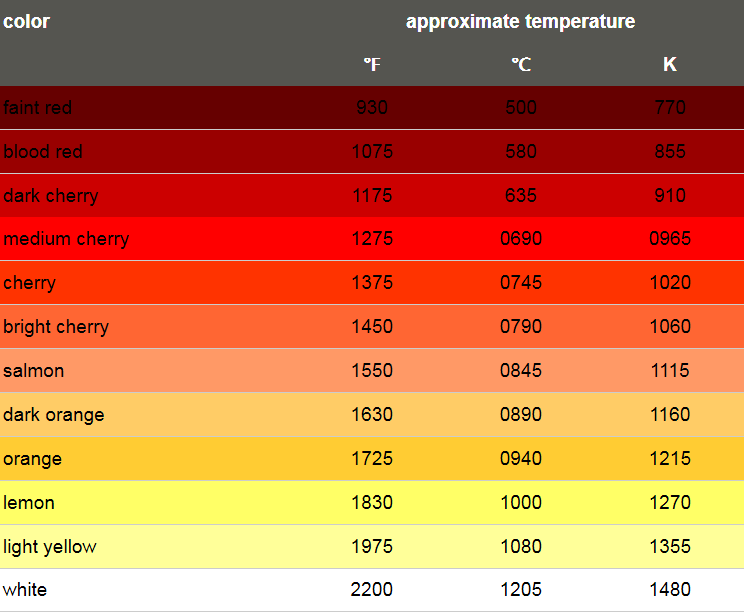
\includegraphics[width=\textwidth]{metalColorTempChart.png}
    \caption{Couleur selon la température}
    \label{fig:couleurTemp}
\end{figure}

\subsection{Élément chauffant}

L'élément chauffant est du nichrome. Ce matériau permet d'atteindre de très grandes températures. La limite est son point de fusion du nichrome qui est d'à peu près 1400 \celsius. La grosseur de fil et la longeur nécessaire dépend de la résistance électrique nécessaire. Elle est calculée selon le voltage disponible et la puissance requise. Pour une puissance de 1200 W,

\begin{equation}
    R = \frac{E^2}{P}
\end{equation}
\[R = \frac{(\SI{120}{V})^2}{\SI{1200}{W}}\]
\[\boxed{R = \SI{12}{\ohm}}\]

La résistance de l'élément doit être de 12 ohm. La résistance électrique d'un métal augmente avec la température.

\var\coeffTNiCr{\SI{.4e-3}{\celsius^{-1}}}

Le coefficient de température de la résistivité $\alpha$ est de \coeffTNiCr pour le nichrome. Le fil est chauffé au maximum à 1400 \celsius.
La résistance de l'élément à cette température serait de

\var\Rref{R_{\rm{ref}}}
\var\Tref{T_{\rm{ref}}}
\begin{equation}
    R = \Rref(1 + \alpha(T - \Tref))
\end{equation}
\[(\coeffTNiCr)(\SI{1400}{\celsius}) = 0.56\]
\[R = 1.56 \Rref\]
\[R = 1.56(\SI{12}{\ohm})\]
\[\boxed{R = \SI{18.72}{\ohm}}\]

ce qui donne une puissance de 769 Watt:

\[P = \frac{E^2}{R}\]
\[P = \frac{(\SI{120}{V})^2}{\SI{18.72}{\ohm}}\]
\[\boxed{R = \SI{769}{Watt}}\]

La résistance $R$ est donné par l'équation,

\begin{equation}
    R = \rho(\frac{L}{A})\Omega
\end{equation}

où $\rho$ est la résistivité du matériau, $L$ est la longeur du fil, et $A$ est l'aire d'une section du fil. La résistivité $\rho$ du nichrome se situe entre \SI{1,0e-6}{\ohm\metre} et \SI{1,5e-6}{\ohm\metre}

Source: https://hypertextbook.com/facts/2007/HarveyKwan.shtml

\todo{Calculer longueur selon l'aire ou l'aire selon la longueur...}

La résistivité de l'acier est de l'ordre de \SI{e-7}{\ohm\metre}. C'est dix fois plus que le nichrome.

\subsection{Temps de chauffe}

L'élément chauffant ne doit pas fonctionner en permanance. S'il était plus gros comme un élément chauffant d'une cuisinière, ce serait possible. Toutefois, pour un petit fil, l'élément doit avoir le temps de dissiper sa chaleur dans l'air.

\todo{Utilisé une résistance variable pour l'instant, c'est trop compliqué les maths, mais je devrais y arriver.}

\newcommand{\uniteCapaciteThermique}{\si{J kg^{-1} \celsius^{-1}}}
La capacité thermique $c$ du nichrome est de 450 \uniteCapaciteThermique. Sa densité $\rho$ est de 8400 \si{kg / m^3}. Le fil de \num{0.5e-3} m de diamètre mesure 1.270 m.

\[m = \pi(\frac{d}{2})^2(l)(\rho)\]
\[m = \pi(\frac{\num{0.5e-3}}{2})^2(1.270)(8400)\]
\[m = \SI{2.1}{g}\]

L'élément nécessite pour se réchauffer

\[(450 \uniteCapaciteThermique)(\SI{0.0021}{kg}) = \]
\[\boxed{\SI{0.945}{J/\celsius}}\]

La puissance de l'élément chauffant diminue avec la température parce que sa résistance augmente. La puissance est donné par l'équation

\[P(T) = \frac{P_0}{1+\alpha(T-\Tref)}\]

\var\Tf{T_{\rm{f}}}
Le temps de chauffe est

\[t(T) = \frac{c(\Tf-T)(m)}{\frac{P_0}{1+\alpha(T-\Tref)}}\]
\[t(T) = \frac{(\SI{0.945}{J/\celsius})(1400\celsius-T)}{\frac{\SI{1200}{W}}{1+\coeffTNiCr(T-20\celsius)}}\]

\subsection{Maintien de la température}

Le chauffage au début n'est pas très important puisque c'est juste quelque secondes. L'important est de bien maintenir la température optimal de l'élément chauffant. Calculer la dissipation de la chaleur de l'élément dans l'air, dans la brique et dans l'environment est hors de mes compétences. Ainsi, une approche expérimentale est utilisée.

Idéalement, un thermomètre serait en contact direct avec l'élément chaufant afin de connaître sa température exact. Le PID pourrait alors controller de manière optimal l'élément.

La puissance de l'élément doit toutefois quand même être déterminer préalablement. Si le puissance est trop élevé, l'élément va chauffer rapidement et vite arrêter. Il risque de surchauffé. Si la puissance n'est pas suffisante, l'élément n'atteindra jamais la température optimale.

Une température de 1000 \celsius est souhaitable.

J'estime, à 100 Watts, ça prends 10-15 secondes avant que l'élément atteigne sa température.

Je ne connais pas le temps de réaction du thermomètre non plus.

\subsection{Température de fusion}

La température la plus élevé possible est souhaitable. Toutefois, elle doit demeurer inférieur à la limite du ciment réfractaire (1473 \celsius).

La température de fusion de certains matériaux.

\begin{table}[ht]
    \caption{Températures de fusions (\celsius)}
    \centering
    
    \begin{tabular}{|c|c|}
        \hline
        aluminium & 660 \\
        cuivre & 1084 \\
        fonte & 1127-1204 \\
        babbitt & 249 \\ 
        \hline
    \end{tabular}
    \label{tab:point_fusions}
\end{table}
Source: \url{https://www.engineeringtoolbox.com/melting-temperature-metals-d_860.html}

\subsection{Seulement l'élément chauffant}

Si on oublie le four. On veut tenir l'élément chauffant à 1000 \celsius.

Je veux faire chauffer mon element hors du four. Je veux du feedback selon le voltage de l'element.

La première étape serait peut-être de faire un circuit avec un potentiomètre. Comme ça je pourrais faire des test préléminaire.

Je vais utiliser mon SSR comme Q1, devrait tenir bon.

Mon SSR peut passer 40A.

L'ampérage d'entrée est de 4-20mA. Trigger à 7.5 mA. Donc 10 mA. Attention c'est du DC.

Je vais pouvoir utiliser mon power supply!

https://cdn.sparkfun.com/datasheets/Components/General/SSR40DA.pdf

Variable Resistance control
Trimmer control method
Power output is controlled by the trigger angle of triac. With variable resistor 250kohm /110VAC

NON, pas phase angle. Phase angle c'est avec AC, et là mon control va être en DC.

Ça me prends un circuit oscillateur avec un pwm.

https://electronics.stackexchange.com/questions/232921/confusion-with-triac-firing-and-zero-crossing-point

Un timer 555 qui va contrôler on/off.

Le voltage minimum du 555 est de 4.5V est max de 16V

Source: https://www.electronics-tutorials.ws/waveforms/555_oscillator.html

Un timer 555 est utiliser pour pouvoir avoir un duty cycle faible pour chauffer l'élément.

\todo{Checker l'ampérage requis pour l'activer aussi. Ça va me donne la résitance de R2}

\begin{figure}
    \centering
    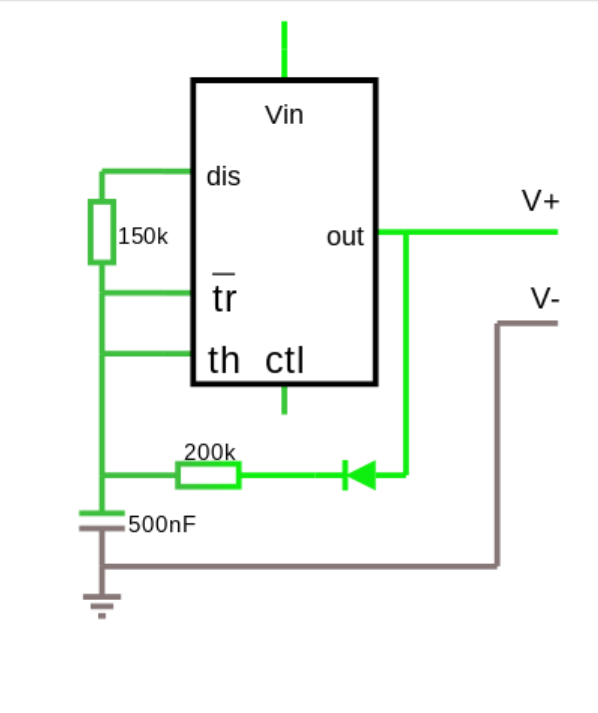
\includegraphics[scale=0.25]{timer555.png}
    \caption{Circuit avec timer LM555}
    \label{fig:my_label}
\end{figure}

\end{document}
